% Workshop-length version. The full treatment is paper/main.tex (14pp).
% This cut is organised around what survived adversarial audit and re-testing, and drops the
% variance decomposition, the lineage analysis (kill condition K5 failed), and the extended
% misspecification simulations. Every number here traces to a JSON artifact in results/.
\documentclass[10pt,letterpaper]{article}
\usepackage[T1]{fontenc}
\usepackage{lmodern}
\usepackage[utf8]{inputenc}
\usepackage{amsmath,amssymb,amsthm}
\usepackage{booktabs}
\usepackage{graphicx}
\usepackage{microtype}
\usepackage[margin=2.5cm]{geometry}
\usepackage[hidelinks]{hyperref}
\usepackage{natbib}

\newtheorem{lemma}{Lemma}

\title{\bfseries Your Diversity Metric Is Measuring Item Difficulty}
\author{Shaurya Gupta\\\small\texttt{shauryaguptaa8@gmail.com}}
\date{\today}

\begin{document}
\maketitle

\begin{abstract}
\noindent
Claims that language models ``fail on the same inputs'' are usually supported by comparing a
pairwise agreement or co-failure rate against an independence baseline. We show that comparison is
uninformative by construction. Mean pairwise co-failure is exactly the \emph{double-fault}
diversity measure of the classifier-ensemble literature \citep{kuncheva2003}, and it is a
deterministic function of the item margins, so its excess over any item-margin-preserving null is
identically zero --- verified to $10^{-16}$ on five benchmarks. We apply the exact conditional
null implied by Rasch sufficiency, following standard nonparametric Rasch methodology
\citep{ponocny2001}, to $1{,}228$--$1{,}373$ open models per benchmark, and --- unlike prior uses
--- we characterise the test's power rather than asserting its validity. Three results follow.
The residual correlation that survives conditioning is $2.9$--$11.9\times$ its null and is
\emph{not} a duplicate-model artifact: removing every model agreeing with a retained model above
$0.95$ discards $36$--$64\%$ of each population and moves $14$ of $15$ headline statistics by less
than $1.5\times$. The test has power $1.00$ against planted shared failure modes at a strength well
below what is observed, and detects copying from a rate of $0.1$. And it has power exactly
$\alpha$ against the alternative in which all models share one item-difficulty profile --- that
alternative \emph{is} the null, so the strongest form of monoculture is invisible to this design
by construction. We state that blind spot as a property, not a caveat. We also show that the
statistic most tempting to report, an ``effective number of independent models,'' is a monotone
function of mean squared residual correlation and counts nothing; the same objection applies to
the Kish design effect used in recent LLM-judge work \citep{kohli2026nine}.
\end{abstract}

\section{The degenerate statistic}

Let $F\in\{0,1\}^{N\times M}$ with $F_{im}=1$ iff model $i$ fails item $m$; write $c_m=\sum_i F_{im}$
and $O=\frac{1}{MN(N-1)}\sum_{i\neq j}\sum_m F_{im}F_{jm}$ for mean pairwise co-failure.

\begin{lemma}\label{lem:mean}
$\displaystyle O=\frac{1}{MN(N-1)}\sum_m\bigl(c_m^2-c_m\bigr)$.
\end{lemma}
\begin{proof}
$\sum_{i\neq j}F_{im}F_{jm}=(\sum_i F_{im})^2-\sum_i F_{im}^2=c_m^2-c_m$ since $F_{im}\in\{0,1\}$.
\end{proof}

$O$ depends on the item margins alone. Any randomisation preserving them leaves $O$ exactly
invariant, so its ``excess over independence'' is identically zero and its standardised effect
size is $0/0$. The scope matters: this follows from preserving \emph{item} margins, so it does not
by itself impugn analyses whose baseline conditions on model accuracy.

$O$ is not an unfamiliar quantity in machine learning --- it is the double-fault measure, one of
the ten catalogued by \citet{kuncheva2003}. The degeneracy is visible in that literature's own
regression design: over $5{,}999$ panels sampled from our ARC response data, mean member accuracy
and panel size alone explain $R^2=0.9928$ of majority-vote accuracy, and the standardised
coefficients on member accuracy and double-fault diverge to $+316$ and $+275$ --- the signature of
the collinearity Lemma~\ref{lem:mean} predicts. Adding both classical diversity measures gains
$\Delta R^2=0.0017$; adding a difficulty-conditioned measure gains $0.0002$, with the wrong sign.
\textbf{Diversity metrics, corrected or not, do not help panel construction at this scale.} This
converges with independent, contemporaneous work: \citet{kim2026diversity} audits five diversity
measures against realised majority-vote gain over $31{,}900$ LLM-ensemble subsets and shows the
same statistics are algebraically rank-deficient once mean accuracy is controlled, by a different
route (no margin-preserving null, gain-over-best-member as target) --- we flag the overlap rather
than claim the finding as ours alone.

The degeneracy has been proved independently in three literatures --- as Schluter's V-ratio in
ecology, Kuder--Richardson/Cronbach's $\alpha$ in psychometrics, and Fleiss's observed agreement
for the multi-category case. We claim the translation, not the result.

\section{The null, and what it can see}

Row and column margins are the jointly sufficient statistics of the Rasch family, so the uniform
distribution over margin-matched matrices is an exact, fit-free conditional null for that family.
This is standard nonparametric Rasch methodology \citep{ponocny2001,verhelst2008}; our
contribution is to apply it at this scale and to characterise it. We sample it with curveball
\citep{strona2014}, which is uniform on the fibre provided failed trades are counted
\citep{carstens2015}.

\paragraph{The sampler is uniform (verified).} Enumerating every binary matrix with given margins
on four fibres (sizes $48$, $90$, $204$, $1170$) and drawing $60{,}000$ thinned samples, a $\chi^2$
test against uniformity is not rejected on any ($p=0.05,0.23,0.73,0.15$). Four dispersed chains
give Gelman--Rubin $\hat R\in[0.98,1.03]$ on all five benchmarks.

\paragraph{The null is not the noise floor.} The exact null's residual-correlation rms sits at
$1.25$--$2.01\times$ the analytic $1/\sqrt{M-3}$ floor. Two rungs are informative: conditioning on
model margins alone lands exactly \emph{on} that floor, while conditioning on item margins alone
reproduces the both-margin null to within $6\%$. Empirically the item margins do essentially all
the conditioning work.

\paragraph{Power, and the blind spot.} On planted data ($400$ models, $700$ items, $20$ datasets
per condition, $\alpha=0.05$; null conditions reject at $0.017$):

\begin{center}\small
\begin{tabular}{lll}
\toprule
planted alternative & strength & power \\
\midrule
shared failure modes & $s=0.3$ / $s=0.5$ & $0.15$--$0.25$ / $\mathbf{1.00}$ (at rms $0.048$) \\
copying a reference model & $c=0.05$ / $c=0.10$ & $0.65$ / $\mathbf{1.00}$ \\
\textbf{shared item difficulty only} & --- & $\mathbf{0.05}=\alpha$ \\
\bottomrule
\end{tabular}
\end{center}

\begin{figure}[t]\centering
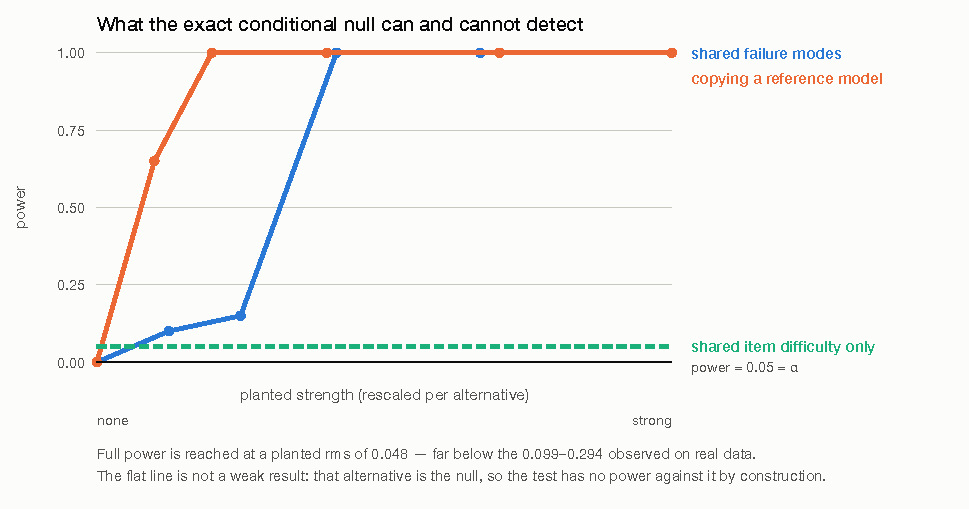
\includegraphics[width=0.92\linewidth]{../figures/fig_power.pdf}
\caption{Detection power against three planted alternatives. The flat line is the design's blind
spot, not a weak result: models sharing one item-difficulty profile and differing only in ability
are exactly what the null describes.}
\label{fig:power}
\end{figure}

Full power is reached at a planted rms of $0.048$, far below the $0.099$--$0.294$ observed
(Figure~\ref{fig:power}). The third row is the Narcissus effect of \citet{colwell1984} in exact
form: if every model finds the
same items hard and differs only in ability, that case \emph{is} the null and the test cannot see
it. A null result here is not evidence of independence. We report this in the abstract because a
reader who does not know it will misread a negative finding.

\section{What survives, on 1,228--1,373 models per benchmark}

Substrate: five benchmarks from the Open LLM Leaderboard v1 archive (July 2023--June 2024),
harvested at zero compute cost by column-selective parquet reads. Residual correlation is the rms
off-diagonal of the margin-conditioned excess matrix.

\begin{center}\small
\begin{tabular}{lrrrrr}
\toprule
& \multicolumn{2}{c}{rms residual correlation} & \multicolumn{2}{c}{after dedup at $0.95$} & dims \\
\cmidrule(lr){2-3}\cmidrule(lr){4-5}
benchmark & observed & vs.\ null & \% removed & ratio & above edge \\
\midrule
ARC-Challenge & $0.2483$ & $5.58\times$ & $36\%$ & $5.44\times$ & $6$ \\
Winogrande    & $0.2691$ & $6.58\times$ & $34\%$ & $6.18\times$ & $5$ \\
TruthfulQA    & $0.2942$ & $5.06\times$ & $40\%$ & $4.64\times$ & $5$ \\
GSM8K         & $0.0987$ & $2.85\times$ & $21\%$ & $3.10\times$ & $4$ \\
HellaSwag     & $0.2457$ & $11.84\times$ & $64\%$ & $13.45\times$ & $12$ \\
\bottomrule
\end{tabular}
\end{center}

\textbf{The effect is not duplication.} This is the objection the population invites, and it does
not hold for the population-level statistics: $14$ of $15$ statistic--benchmark pairs move by less
than $1.5\times$ between the full and $0.95$-deduplicated populations (the exception is
HellaSwag's participation ratio, $2.44\times$). It \emph{does} hold for a gradient claim we
therefore do not make: apparent redundancy concentrating among the highest-accuracy models
collapses under the same deduplication on three of five benchmarks.

\textbf{Dimensionality.} Counting eigenvalues above the null spectral edge is Horn's parallel
analysis with a stronger reference than Horn's own --- the exact margin-preserving null already
carries the observed ability and difficulty profiles. Retained counts are $4$--$6$ ($12$ on
HellaSwag), stable to within one across deduplication thresholds on four of five benchmarks. These
are upper bounds; eigenvalue-counting rules over-retain. This bears directly on IRT-based
benchmark compression \citep{polo2024tiny}, which fits latent-ability models to matrices of this
kind --- using $319$ models, roughly a quarter of the population here --- and rests on an assumed
dimensionality. Our test needs no IRT fit of its own, so it can check that assumption.

\section{What we do not claim}

We do \emph{not} report an ``effective number of independent models.'' The participation ratio is
algebraically $N/(1+(N-1)\overline{R_{ij}^2})$, a monotone function of the mean squared residual
correlation, so it cannot distinguish one weak global factor from many tight clusters. The same
objection applies to the Kish design effect $k/(1+(k-1)\bar\phi)$ used as the headline statistic in
recent LLM-judge panel work \citep{kohli2026nine}, differing only in using the mean rather than
the mean square. \citet{benchscope2026} apply the identical participation-ratio statistic on the
orthogonal axis --- counting effective independent \emph{benchmarks} rather than models --- and
reach the same conclusion by a different argument, explicitly treating it as a screening
diagnostic rather than a literal factor count.

The central limitation is identification: our conditioning family is unidimensional, and we cannot
separate genuine behavioural concentration from the Rasch family being too small. A pre-registered
test on real responses found that our own critique does \emph{not} rescue a specific published
claim --- the accuracy--agreement association attenuates only $12\%$ under conditioning --- and we
report that prior finding as robust. A pre-registered dispersion statistic was refuted by its own
kill condition, and a lineage decomposition was dropped when its coverage gate failed at $23.3\%$
against a $40\%$ threshold. All code, substrate, results artifacts and the pre-registration with
dated amendments are released; every number above traces to an executed run.

\paragraph{Use of AI assistance.} A large language model was used as a coding and analysis
assistant. The author directed the research, pre-registered the hypotheses and kill conditions,
verified the derivations, and takes full responsibility, in line with COPE guidance that AI tools
cannot be authors.

\small
\bibliographystyle{plainnat}
\begin{thebibliography}{9}
\bibitem[Carstens(2015)]{carstens2015} C.~J. Carstens. Proof of uniform sampling of binary matrices with fixed row sums and column sums for the fast Curveball algorithm. \emph{Physical Review E}, 91:042812, 2015. Erratum: 94:039902, 2016.
\bibitem[Colwell \& Winkler(1984)]{colwell1984} R.~K. Colwell and D.~W. Winkler. A null model for null models in biogeography. In \emph{Ecological Communities: Conceptual Issues and the Evidence}, 344--359. Princeton University Press, 1984.
\bibitem[Kim(2026)]{kim2026diversity} D.~Kim. Are diversity metrics measuring diversity? A capability-controlled audit of majority-vote gain in LLM ensembles. \emph{arXiv:2607.20768}, 2026.
\bibitem[Kohli(2026)]{kohli2026nine} G.~Kohli. Nine judges, two effective votes: Correlated errors undermine LLM evaluation panels. \emph{arXiv:2605.29800}, 2026.
\bibitem[Kuncheva \& Whitaker(2003)]{kuncheva2003} L.~I. Kuncheva and C.~J. Whitaker. Measures of diversity in classifier ensembles and their relationship with the ensemble accuracy. \emph{Machine Learning}, 51(2):181--207, 2003.
\bibitem[Polo et al.(2024)]{polo2024tiny} F.~M. Polo, L.~Weber, L.~Choshen, Y.~Sun, G.~Xu, and M.~Yurochkin. tinyBenchmarks: evaluating LLMs with fewer examples. \emph{arXiv:2402.14992}, 2024.
\bibitem[Ponocny(2001)]{ponocny2001} I.~Ponocny. Nonparametric goodness-of-fit tests for the Rasch model. \emph{Psychometrika}, 66:437--460, 2001.
\bibitem[Sha \& Zhao(2026)]{benchscope2026} T.~Sha and S.~Zhao. BenchScope: How many independent signals does your benchmark provide? \emph{arXiv:2603.29357}, 2026.
\bibitem[Strona et al.(2014)]{strona2014} G.~Strona, D.~Nappo, F.~Boccacci, S.~Fattorini, and J.~San-Miguel-Ayanz. A fast and unbiased procedure to randomize ecological binary matrices with fixed row and column totals. \emph{Nature Communications}, 5:4114, 2014.
\bibitem[Verhelst(2008)]{verhelst2008} N.~D. Verhelst. An efficient MCMC algorithm to sample binary matrices with fixed marginals. \emph{Psychometrika}, 73:705--728, 2008.
\end{thebibliography}

\end{document}
